% ----
% COMP1204 CW1 Report Document
% ----
\documentclass[]{article}

% Reduce the margin size, as they're quite big by default
\usepackage[margin=1in]{geometry}
\usepackage{listings}
\usepackage{minted}
\usepackage{graphicx}

\title{COMP1204: Data Management \\ Coursework One: Hurricane Monitoring }
% Update these!
\author{Lukas Hjortenfeldt\\ 32890818}

% Actually start the report content
\begin{document}

% Add title, author and date info
\maketitle

\section{Introduction}
My task for this coursework was assigned as such: 
\\I work as a data scientist for the National Oceanographic and Atmospheric Administration Centre (NOAAC) and were assigned to the team of tropical cyclone tracking, tasked with extracting storm data from reports (written in .kml format) given on tropical cyclones and then using that data to plot maps of the storm's location. The data that I extracted was written to a .csv file in order to be processed by the storm plotting bash script (create\_map\_plot.sh).
\\The data I was tasked with extracting from these wordy reports was:
\begin{enumerate}
    \item Storm Latitude: The North/South position of the storm.
    \item Storm Longitude: The East/West position of the storm.
    \item Minimum Sea Level Pressure: The minimum air pressure of the storm, reported in millibars (mb).
    \item Maximum Intensity: The maximum velocity of the winds in the storm, reported in knots.
\end{enumerate}

\newpage
\section{Create CSV Script}
Below is the bash script that I wrote and used to extract the necessary information from the .kml files:

\begin{listing}[h!]
    \begin{minted}[breaklines]{bash}
#!/bin/bash
#Bash script to sort through hurricane data presented in a kml type file and filter out the important components to then store in a csv file.

grep 'UTC\|N,\|mb\|knots' $1 | #search through the input file for the keywords:"UTC", "N,", "mb" & "knots".
sed 's/<[^>]*>//g' | #removes all characters in between any two tags (<*>).
sed 's/\;.*$//g' | #remove all other unnecessary data which comes after all ';' in the file.
sed 's/[ \t]*//' | #format data correctly by removing all tabs from shell output
uniq | #deletes all duplicate lines
awk '!(NR%5==1)' | #removes every 5th line from shell output, as these lines contained additional unncessary duplicate data 
awk '0!=NR%4{$0=$0","} 1' | #add a comma to every line except the 4th ones
sed ':a;/,$/{N;s/\n//;ba}' | #merge all relevant data in one cycle of hurricane into a single line by merging lines together that end in a comma
sed -e 's/ -/-/g' -e 's/ ,/,/g' | #remove whitespace behind negative signs & commas
sed '1 i\Timestamp,Latitude,Longitude,MinSeaLevelPressure,MaxIntensity' > $2 #add relevant text to first line of shell output and pipe into output path file

    \end{minted}
    \caption{Bash script 'create\_csv.sh'}
    \label{lst:hello}
\end{listing}

Thankfully, only the relevant data appeared first before each semi-colon, which is why the third \emph{sed} command worked, as all the other information behind the semi-colons was unnecessary data.

\section{Storm Plots}

\begin{figure}[H]
    \centering
    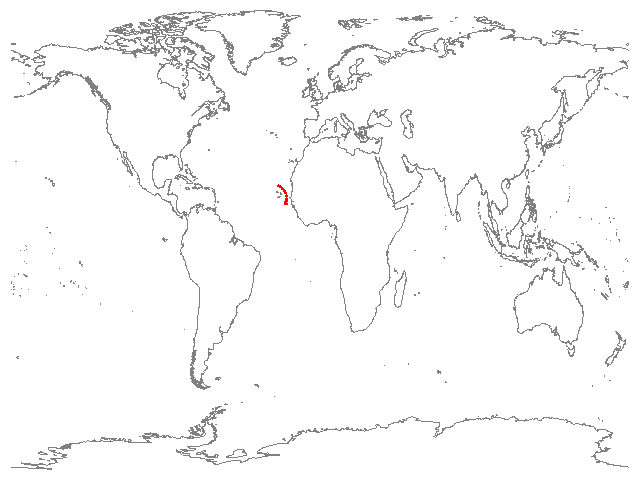
\includegraphics[height = 6cm, width = 12cm]{stormPlot1.png}
    \caption{Plot of storm from kml file: al102020.kml}
\end{figure}
\begin{figure}[H]
    \centering
    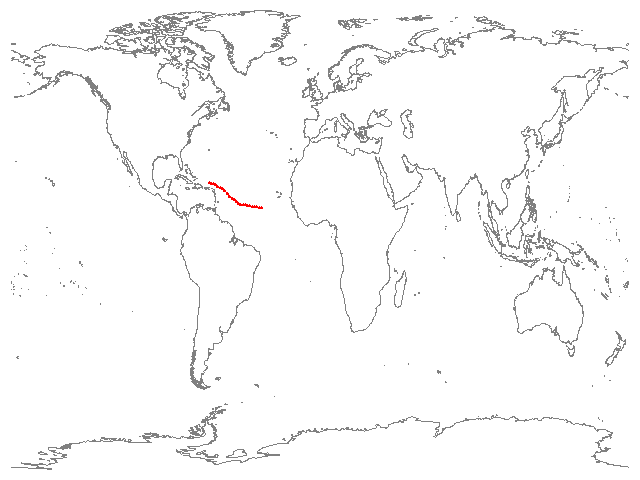
\includegraphics[height = 6cm, width = 12cm]{stormPlot2.png}
    \caption{Plot of storm from kml file: al112020.kml}
\end{figure}
\begin{figure}[H]
    \centering
    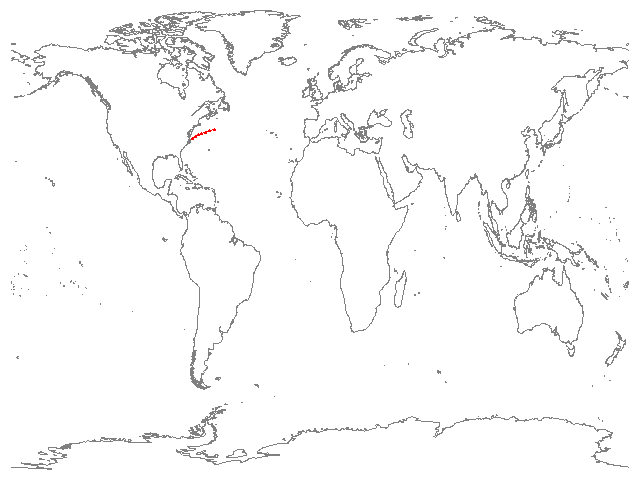
\includegraphics[height = 6cm, width = 12cm]{stormPlot3.png}
    \caption{Plot of storm from kml file: al122020.kml}
\end{figure}

\end{document}